\chapter{绪论}
\label{cha:intro}
\section{研究背景与研究意义}
\label{sec:backgroundandsignificance}
\subsection{研究背景}
\label{sec:research_background}
增强现实(~Augmented Reality,简称AR~)是指透过摄影机影像的位置及角度精算并加上图像分析,让屏幕上的虚拟世界能够与现实世界场景进行结合与互动的技术\footnote{节选自:https://zh.wikipedia.org/wiki/增强现实}。
该项技术是对现实世界环境的实时视图,其通过多种传感器的配合,生成“增强”的视觉信息,并且与物理世界在空间上对齐,从而在现实场景中叠加虚拟化图像。增强现实技术已被各国政府列为重点发展领域,美国政府早在~2000~年制定的《长期核技术研发规划》
中明确提出应重点开发、应用和验证虚拟现实和增强现实技术;其后美国微软(~Microsoft~)公司于~2015~年发布了全球首款头戴式全息增强现实眼镜~Hololens,真正将该项技术带入消费市场;
日本政府在~2014~年公布的至~2025~年技术发展规划《创新~25~战略》中将虚拟现实与增强现实视为技术创新重点方向;韩国政府于~2016~年设立了约~2~亿~4000~万人民币的专项基金,用于发展虚拟现实和增强现实的
研究和发展中。在我国,各级政府积极推动虚拟现实以及增强现实技术的发展,该技术已被列入“十三五”信息化规划、中国制造~2025~、互联网+~等多项国家重大文件中,工信部、发改委、科技部、文化部、商务部出台相关政策,至~2016~年底,我国近二十个省市地区开始
布局专项产业以推动该技术的发展与普及\cite{ZhongguoxinxitongxinyanjiuyuanXuNiZengQiangXianShiBaiPiShu2017}。

AR~技术能够结合实际需求,实现超越现实感官的体验。该技术能够在真实环境中灵活地显示虚拟数据以及图像信息,对客观目标进行实时状态查看并帮助用户及时
处理决策,因此被广泛应用于医疗、建筑、教育、工业维修等领域。全球购物网站亚马逊公司开发的~AR View~系统通过增强现实技术将虚拟商品图像叠加于手机拍摄场景中,如图~\ref{fig:amazonshopping}~所示,用户能够通过该软件更加直观地观察商品的外形,
帮助挑选与周围环境搭配合理的商品;美国卡特(~CAT~)公司使用该技术指导操作人员对机械油路压力系统进行检修,如图~\ref{fig:catfig}~所示,工作人员通过~AR~眼镜可以直观地看到机械油路部件的工作
状态,以及油路压力,降低检修难度;增强现实技术在教育领域也大有可为,如图~\ref{fig:education}~所示\footnote{摘自谷歌图片},该系统由国外独立团队开发,通过识别指定图片特征,在真实场景中叠加
生物结构模型,用于展示不同生物的体貌特征,能够将最直观细致的立体信息展现给用户,传递相较于传统书面教育更多的细节信息,大大提升教育的趣味性。

\begin{figure} %[h]
  \centering%
  \subcaptionbox{亚马逊虚拟购物软件\label{fig:amazonshopping}}{%    
    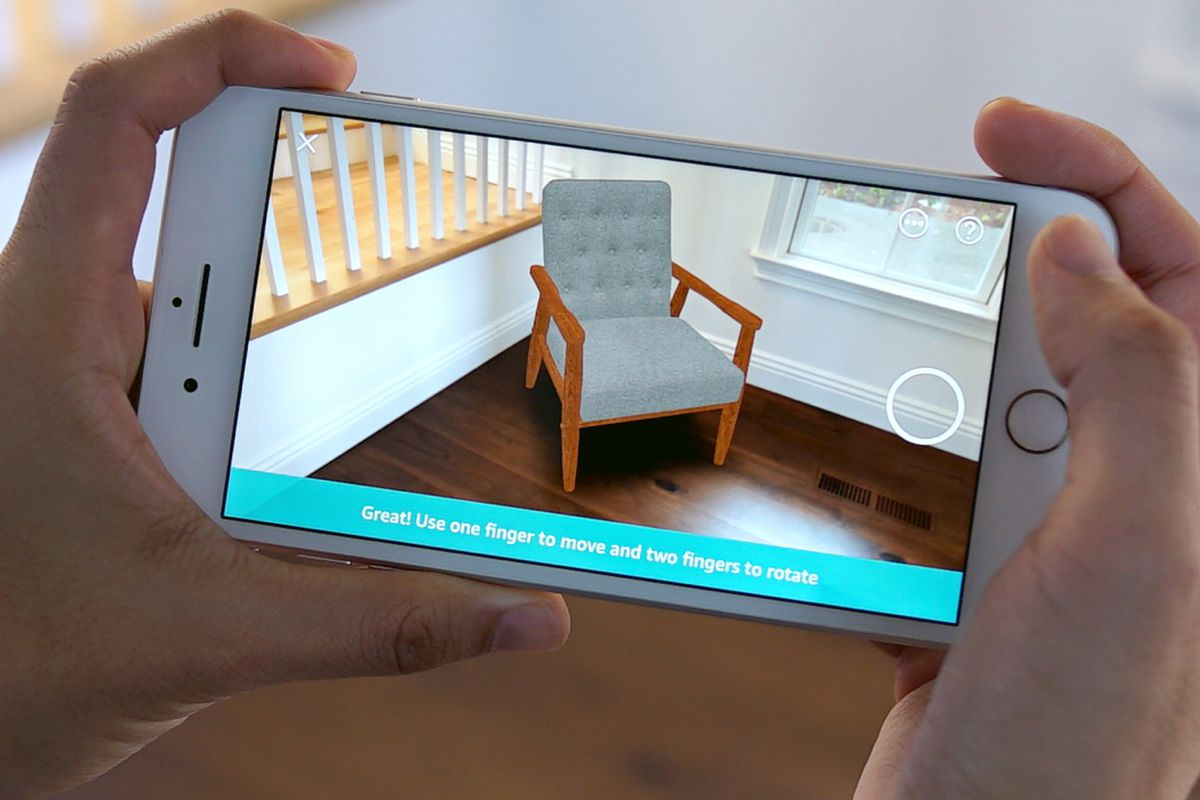
\includegraphics[height=4cm]{1_ARView}} \hspace{1em}
  \subcaptionbox{卡特公司油路检修系统\label{fig:catfig}}{%  
    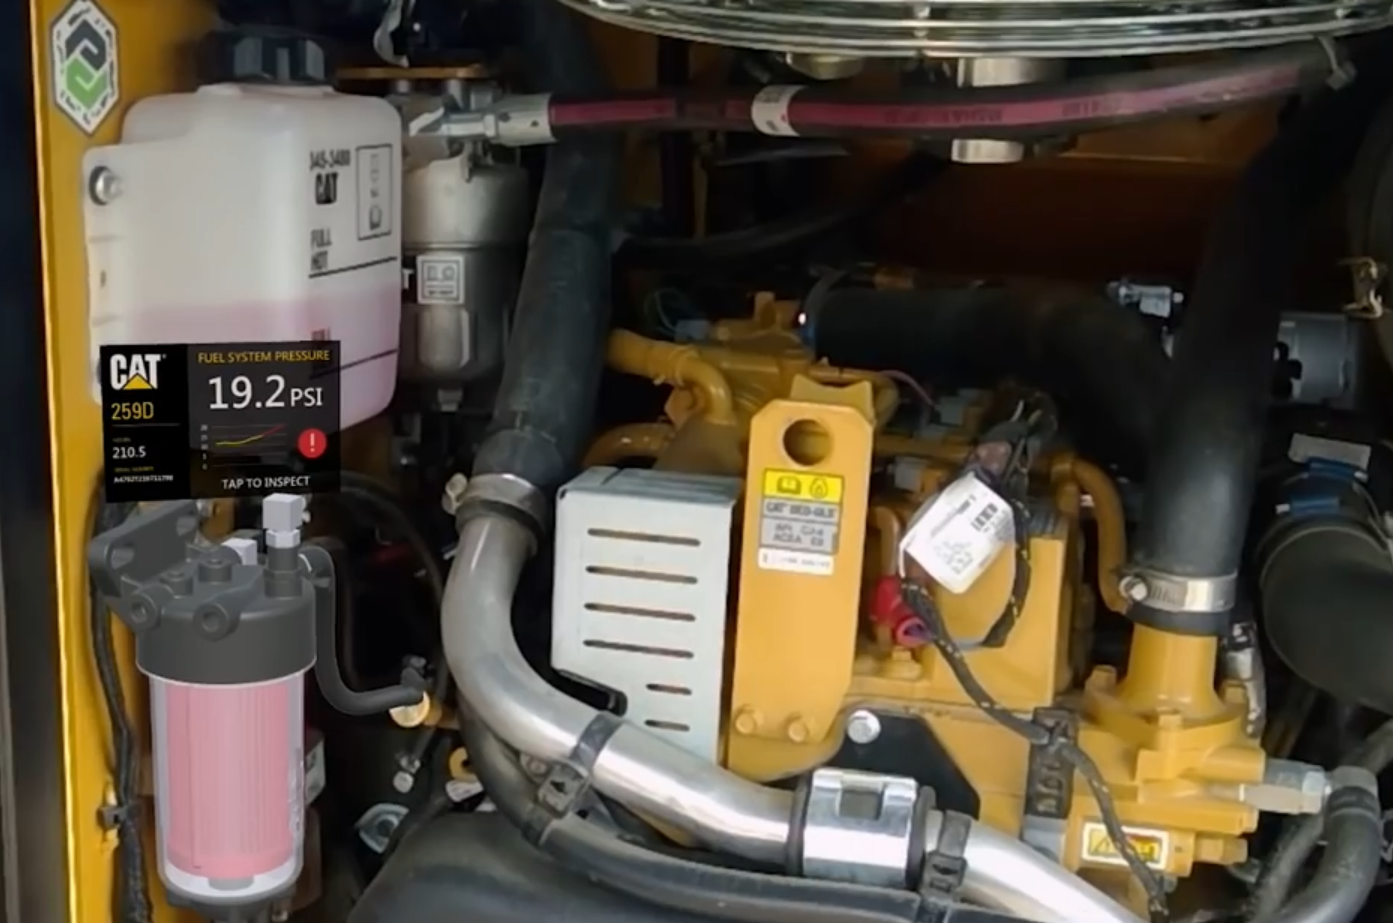
\includegraphics[height=4cm]{1_AR1}
    }\vskip0.3cm%
  \subcaptionbox{生物研究系统\label{fig:education}}{%    
    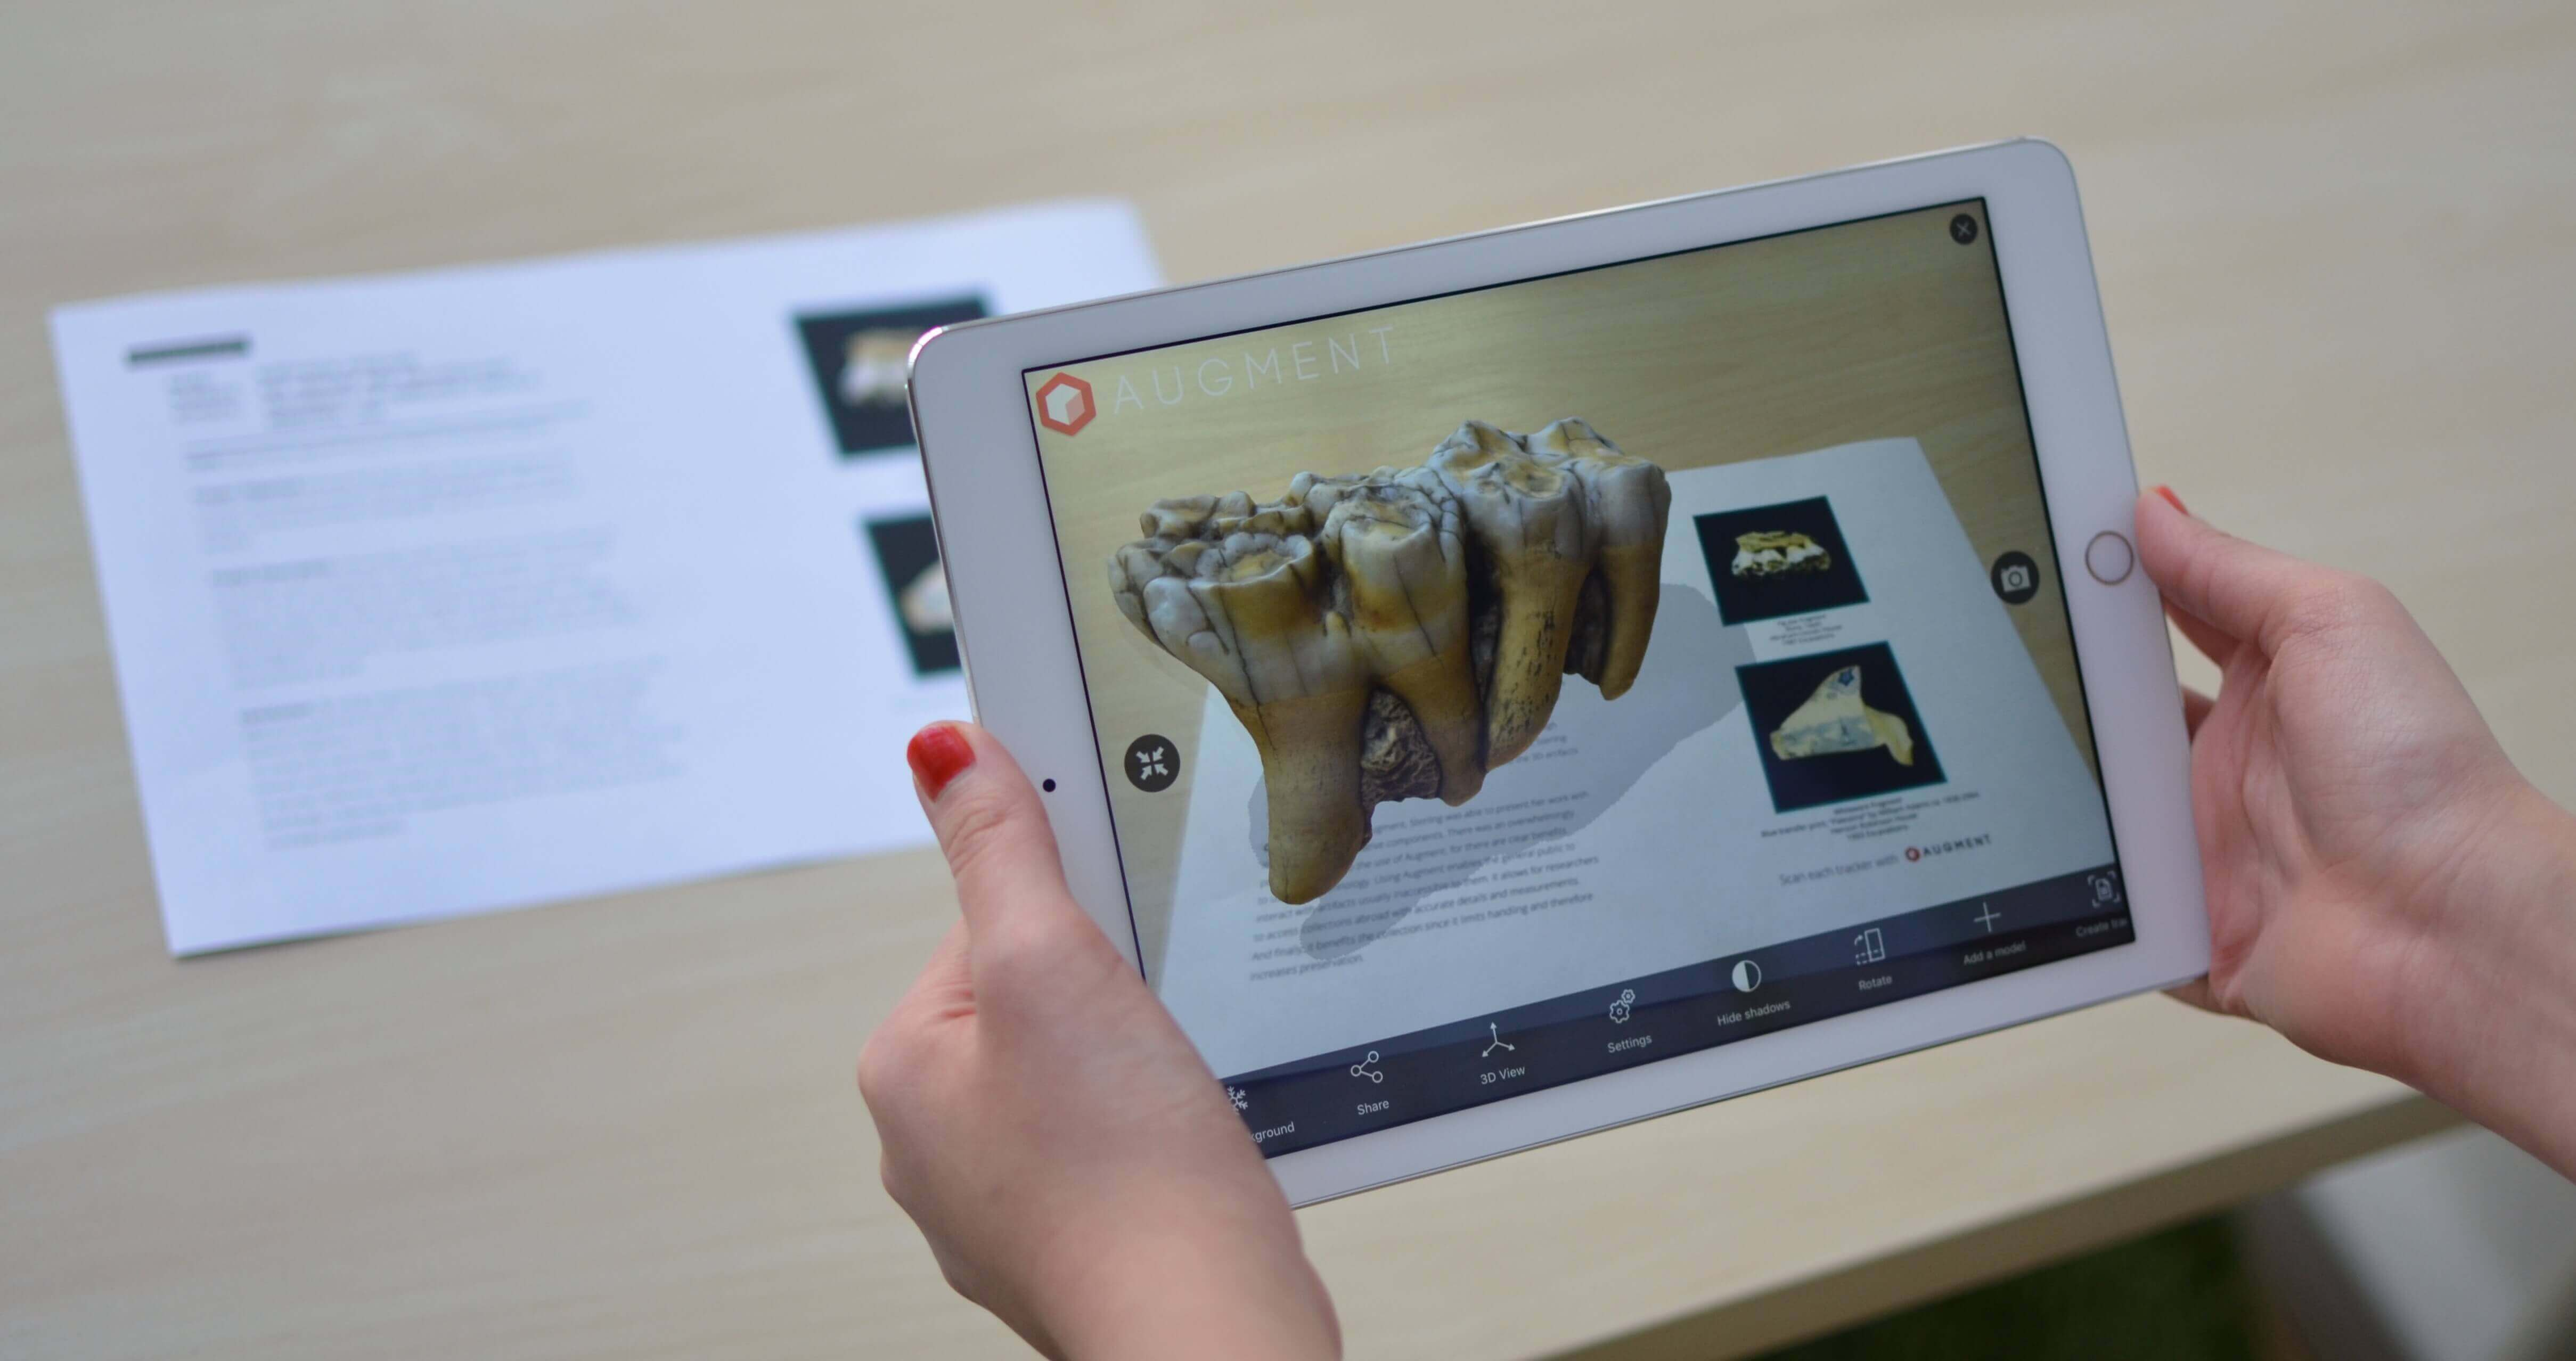
\includegraphics[height=6.8cm]{1_education}}
  \caption{增强现实应用}
  \label{fig:model_based_tracking_example}
\end{figure}


\subsection{研究意义}
\label{sec:significance}
增强现实技术能够直观地指导操作人员、便捷地查看设备运行状态,因此在工业界也将有很多应用,
如在海上风电场检修、电厂高压倒闸等。在条件恶劣、干扰严重、误操作危险的场景中,当需要进行连续多步骤操作时,无法保证人员操作的正确性;并且在操作员学习阶段,如果仅通过书本以及口头传授的方式,
无法获得具体的实践经验,易在实际操作时失误而导致无法挽回的损失。若使用增强现实技术在操作设备上叠加虚拟指导信息,不仅能够在人员操作时进行实时提醒,还能在学习阶段结合理论知识进行实际操作展示,
使学习者更快更清楚地理解操作的意义以及步骤\cite{CaiZengQiangXianShiARZaiJiaoXueZhongDeYingYongAnLiPingShu2017}。

当前广泛使用的~AR~目标物多为表面纹理丰富的物体,在工业上的应用也是依靠张贴图片目标帮助进行定位。针对该类应用场景,
采用基于物体表面特征点的追踪方法已能满足精度要求\cite{AhmedImprovedPerturbObserve2015}。
然而在工业生产领域,目标物多为金属材料,表面光滑贫纹理,无法使用特征点跟踪方法实现精确定位与追踪,并且使用张贴目标图像帮助定位的方法将限制工件的运动范围,而且定位精度较低,对使用效果有较大影响,
该缺陷很大程度上限制了~AR~技术在工业上的应用\cite{RanXuNiXianShiJiZengQiangXianShiJiZhuZaiGongYeSheJiZhongDeYingYong2010,LiuARJiZhuZaiQiCheGongYeLingYuDeYingYong2017}。

因此贫纹理作业目标精确定位与追踪系统需要使用目标物体的三维模型信息对物体实现六自由度的追踪。系统应保证在复杂背景下目标姿态位置检测追踪的精确度以及稳定度,还需要在一定程度上降低算法的复杂度,
确保系统的快速性。该系统不仅能够扩大~AR~技术的适用范围,还能在工业抓取、装配领域起到辅助定位的效果,因此对该系统的研究具有十分重要的工程意义。




\begin{comment}
\begin{figure}[b] %[h]
  \centering%
  \subcaptionbox{亚马逊分拣大赛\label{fig:picking}}{%    
    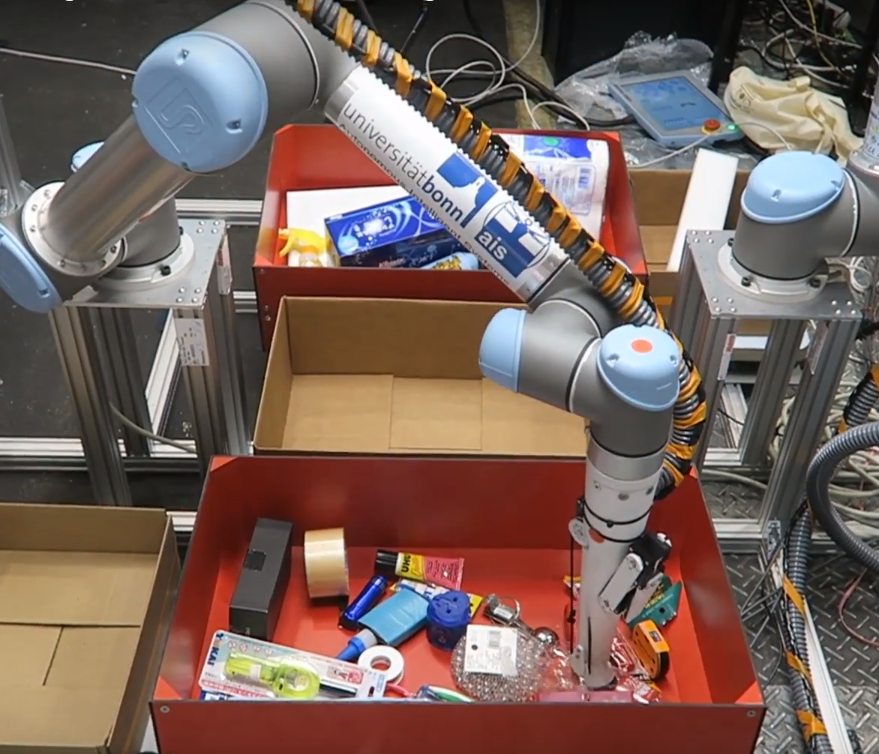
\includegraphics[height=7cm]{1_robot.png}\hspace{1em}
    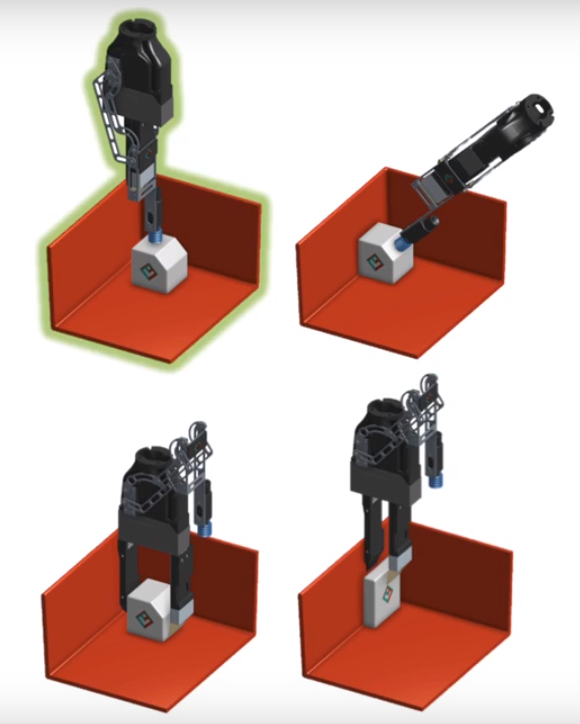
\includegraphics[height=6cm]{1_picking2.png}
    }\vskip0.3cm%
  \subcaptionbox{增强现实\label{fig:vuforia}}{%    
    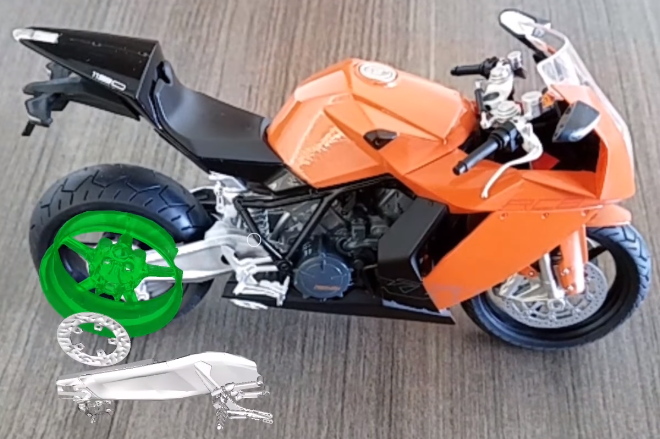
\includegraphics[height=7cm]{1_vuforia.png}}
  \caption{目标位姿追踪}
  \label{fig:model_based_tracking_example}
\end{figure}


高精度目标物体姿态追踪系统在工业生产以及增强现实领域应用广泛。如美国亚马逊公司开创设立的部件分拣大赛,自2015年开始吸引来自世界各地的优秀工业视觉团队,使用视觉识别方法联合机械臂对不同部件实现分拣。
如图\ref{fig:picking}所示,来自澳大利亚机器人视觉中心的团队在十六支队伍中脱颖而出获得冠军,其机械臂依靠视觉定位算法能够分拣出50余种不同形状的物体。至今还未有国内团队在该项大赛上取得好成绩。增强现实
技术效果如图\ref{fig:vuforia}所示,通过定位目标物体相对于相机的位姿,叠加指导性的虚拟图像以展示部件的组成,效果直观。

UNIX~操作系统(UNIX),是美国AT\&T公司1971年~在PDP-11上运行的操作系统。具有多用户、
多任务的特点,支持多种处理器架构,最早由肯·湯普遜(Kenneth Lane Thompson)、
丹尼斯·里奇(Dennis MacAlistair Ritchie),见图\ref{fig:ken}。和~Douglas
McIlroy~于1969年在~AT\&T~的贝尔实验室开发\footnote{摘自中文维基百科}。\par
\begin{figure}[htbp]
    \centering
	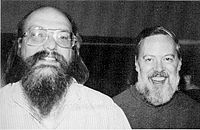
\includegraphics{Ken_n_dennis}
    \caption{肯·汤普逊(左)和丹尼斯·里奇(右)}
    \label{fig:ken}
\end{figure}
Linux~操作系统(Linux),是一类计算机操作系统的统称。Linux~操作系统的内核的名字也是~“Linux”。
Linux~操作系统也是自由软件和开放源代码发展中最著名的例子。严格来讲,Linux~这个词本身只表
示~Linux~内核,但在实际上人们已经习惯了用~Linux~来形容整个基于~Linux~内核,并且使用~GNU~
工程各种工具和数据库的操作系统(也被称为~GNU/Linux~)。基于这些组
件的~Linux~软件被称为~Linux~发行版\cite{LoweDistinctiveimagefeatures2004}。

Linux内核最初只是由芬兰人林纳斯·托瓦兹(Linus
Torvalds),见图\ref{fig:linus},在赫尔辛基大学上学时出于
个人爱好而编写的,当时他并不满意~Minix~这个教学用的操作系统,部分因为只能在有限硬件上运行。
最初的设想中,Linux~是一种类似~Minix~这样的一种操作系统。Linux~的第一个版本在1991年9月
被大学~FTP server~管理员~Ari Lemmke~发布在~Internet~上,最初~Torvalds~称这个内核的名称为
~"Freax",意思是自由("free")和奇异("freak")的结合字,并且
附上了~"X"~这个常用的字母,以配合所谓的~Unix-like~的系统。但是~FTP server~管理员
嫌原来的命名~“Freax”~的名称不好听,把内核的称呼改成~“Linux”~,当时仅有10000行代码,仍必须
运行于~Minix~操作系统之上,并且必须使用硬盘开机;随后在10月份第二个版本(0.02版)
就发布了,同时这位芬兰赫尔辛基的大学生在~comp.os.minix~上发布一则消息\par
\begin{center}
\fbox{\parbox[t]{0.8\textwidth}{
Hello everybody out there using minix-\\
I'm doing a (free) operation system (just a hobby,\\
won't be big and professional like gnu) for 386(486) AT clones.}}
\end{center}
\begin{figure}[htbp]
    \centering
    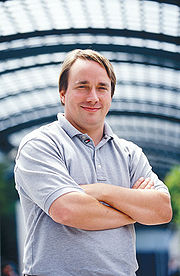
\includegraphics{Linus_Torvalds}
    \caption{Linus Torvalds}
    \label{fig:linus}
\end{figure}
\end{comment}

\section{国内外研究现状}
\label{sec:status}

\subsection{目标位姿数据库研究现状}
\label{sec:databasestatus}
带有真值的数据是学习类算法的模板和基础。目标物体位置姿态数据库应至少包含:目标物体三维模型、目标物体场景图像、目标物体相对于相机的姿态变换以及平移向量。该类数据库区别于一般的图像数据库,
其真值无法由图像信息标注获取,只能依靠深度传感器以及陀螺仪进行测量,由此会引入更多测量误差。本节将介绍目前已有的几种目标位姿数据库的生成方法及特点,并进行分析。
\vskip0.2cm

\noindent\textbf{ISY~数据库}\cite{VikstenComparisonLocalImage2009}:

该数据库是由美国纽约长岛大学计算机视觉实验室于 2009 年建立,包含~16~个目标物体,每一个物体都被放置在图像的中间位置,以~5$^\circ$~为步进按照各旋转轴进行旋转。在每一种姿态下,通过模型渲染将目标物体叠加于背景之上,
背景包含全黑的虚拟简单背景以及真实照片的复杂背景。该数据库设置目标物体处于相机视野的正中间,即固定了目标物体相对于相机的平移向量;之后再通过等间距地改变物体的姿态以生成环视图片集。数据库生成方法较为简单,
但适用范围较小,仅能用于物体检测并分割后的姿态判定算法训练,还须保证分割图像中物体的比例与数据库中接近。并且该数据库并不是放置在真实世界中的目标物体图像,而是基于物体模型的渲染与真实
世界背景的叠加以获得的合成图片。该方法虽能保证姿态真值的可靠性,但在合成图像的边界处存在不真实过渡的现象,导致在物体检测和分割算法中误差较大。加之该数据库不含连续视频帧的图像,因此也无法用于追踪算法精度的测试。

\vskip0.2cm
\noindent\textbf{ACCV~数据库}\cite{HinterstoisserGradientResponseMaps2012}:

该数据库由德国慕尼黑工业大学于 2012 年完成,包含超过~18000~张真实图片,涵盖~15~种不同的物体在多种环境中的位姿真值与对应图像。其中包含物体的三维点云模型、场景的~RGB~图像以及深度图像、物体的位姿真值、以及采集图片所用相机的参数等。数据库较为完善且精度较高,被很多算法
作为训练的资源。但该数据库使用视觉算法估计位姿,无法确定该位姿真值的可信度以及误差的大小,因此无法作为算法评价标准,而且该数据库缺少连续视频帧图像,无法用于追踪算法的精度测试。

\vskip0.2cm
\noindent\textbf{ICVL~数据库}\cite{DoumanoglouRecovering6DObject2015}:

ICVL~数据库是由伦敦帝国学院计算机视觉实验室于~2016~年制作,该数据库使用陀螺仪的测量方式确定每一张图像中物体与相机的相对位姿,该方法使用非视觉传感器测量目标物体相对相机的位置和姿态,提高了真值的可信度。
数据库中包含~6~种常见的商品包装盒作为检测目标,包含物品的三维模型、~RGB~图像以及深度图像。但该数据库模型较少,而且多为矩形物体,无法使用该数据库评估复杂模型检测与追踪算法的精度。
虽然数据库中含有多个场景拍摄的目标物体图像,但仍然不是连续的视频帧图像,无法用于姿态追踪算法的精度测试。

\vskip0.2cm
\noindent\textbf{ObjectNet~3D~数据库}\cite{XiangObjectnet3dLargeScale2016}:

该数据库由斯坦福大学计算机视觉实验室建立,其中包含~9~万余张真实场景图像,使用人工对齐方法获得物体在场景中的位姿。该数据库所提供的模型并没有与现实场景中的物体完全匹配,而是按照物体类别进行粗匹配。
该方法减少了模型的数量,因此数据库建立的难度也同时降低,但人工标注的方法无法保证位姿真值的可靠性,并且模型粗匹配也将导致基于模型的追踪方法精度降低。因此该数据库一般用于物体的检测和分类,而姿态信息仅作为
检测精确度的度量。

\subsection{目标物体检测与姿态定位研究现状}
\label{sec:detection_status}
基于特征点匹配的目标检测与位姿估计起步较早,其核心理论~$P3P$~算法可以追述到二十世纪九十年代。该方法要求至少能
在单张图像中匹配定位 4 个物体特征点,并确定与特征点相对应的目标模型三维空间点,依据单目相机投影模型
计算三维空间点在图像中的投影点,迭代优化使得投影点与~2D~特征点距离最小,由此得到目标物体
相对于相机的旋转矩阵以及平移向量。该算法使用特征点提取与匹配寻找两维图像点与三维物体表面特征点对应关系,由此实现目标物体的检测与位姿判定。
中国科学院沈阳自动化研究于 2006 年提出的一种基于线的 $PnP$ 方法通过识别物体表面三条互相垂直的直线,求解物体相对于相机姿态的方法\cite{QinYiChongQueDingWuTiZiTaiDeBiShiJieFangFa2006},提高了姿态估计的精度,并且算法速度较快,效果良好。
该方法存在很多优化的方向,主要有特征点的选取\cite{NayarRealtime100Object1996,ViolaRapidObjectDetection2001,SkrypnykSceneModellingRecognition2004,JiaJiYuJiHeGuanXiYueShuDeTeZhengDianPiPeiSuanFa2015}、滤波算法\cite{LoweObjectRecognitionLocal1999,MikolajczykAffineInvariantInterest2002,YiJiYuTeZhengDianDeTuXiangPeiZhunJiQiZaiWenXiangZhongDeYingYong2013}、迭代优化\cite{LuFastGloballyConvergent2000,AnsarLinearPoseEstimation2003,GaoCompleteSolutionClassification2003}等做出改进。
直到~2009~年由~Lepetit~等人提出的~$EPnP$~算法\cite{LepetitEpnpAccurateSolution2009}将图像坐标中的
特征点作为~4~个假设点的权值,通过矩阵计算求解最小误差以获得目标位姿的方法,将该类匹配算法的复杂度降低到~$O(n)$~.

随着硬件计算能力的提高,特征点的数量对算法效率的影响逐渐减少。于 2014 年之后出现了大量基于机器学习方法提取目标物体特征点描述子的匹配算法,使用抽象高阶特征匹配计算物体位姿\cite{GirshickRichFeatureHierarchies2014,GaninUnsupervisedDomainAdaptation2014,GengJiYuTouShiBuBianErZhiTeZhengMiaoShuZiDeTuXiangPiPeiSuanFa2015,HuDeepTransferMetric2015,RadFeatureMappingLearning2017,RozantsevSharingWeightsDeep2018}。
该类算法通常需要两个网络进行位姿判断;首先是特征提取网络:输入为~2D~图像,输出为特征描述子,该网络将图像空间映射到特征空间,训练阶段需要输入含有目标物体的图片正样本以及不含物体的负样本,通过特征提取与匹配方法
判断当前场景是否存在目标物体;其后是位姿判断网络:输入为特征描述子,输出为目标物体相对于相机的位姿,该网络通过当前特征描述子解算物体的旋转矩阵以及平移向量。该网络的训练可以使用
虚拟数据库,根据目标物体三维模型,自动布置相机位置并生成图片\cite{HinterstoisserPreTrainedImageFeatures2017,KehlSSD6DMakingRGBbased2017}。该方法相比其他学习方法网络结构较为简单,训练成本较小;但受特征提取影响较大、
准确度较低,很难实现精确追踪。

\begin{comment}
UNIX~的历史开始于1969年~ken Thompson,Dennis Ritchie~(即著名的~K\&G~,~C~语言的发明人)
与一群人在一部~PDP-7~上进行的一些工作,后来这个系统变成了~UNIX。\par
主要大事件:
\begin{itemize}
    \item V1(1971):第一版的UNIX,以~PDP-11/20的汇编语言写成。
        包括文件系统,~fork、roff、ed~等软件。
    \item V4(1973):以~C~语言从头写过,这使得~UNIX~修改容易,可以在几个月内移
        植到新的硬件平台上。最初C语言是为~UNIX~设计的,所以~C~与~UNIX~间有紧密的关系。
    \item V6(1975):第一个在贝尔实验室外(尤其是大学中)广为流传的~UNIX~版本。
        这也是~UNIX~分支的起点与广受欢迎的开始。1.xBSD (PDP-II)就是由这个版本衍生出来的。
    \item V7(1979):在许多UNIX玩家的心目中,这是“最后一个真正的~UNIX,”
        这个版本包括一个完整的~K\&RC~编译器,Bourne
        shell。V7~移植到~VAX~机器后称为~32V。
\end{itemize}
基于模型的视觉追踪算法根据特定物体的三维特征,在二维图像中寻找对应关系。该类方法最早出现在上世纪九十年代早期,通过在二维图像空间中寻找位置以及方向匹配信息,实现目标物体在图像
平面的对齐,具体配准过程是对位置方向匹配方程的寻优。该类方法不再依靠图像特征点,一般通过提取图像的边缘作为匹配的特征,适用范围更广,鲁棒性更高。本论文的研究对象贫纹理作业目标是
一种表面特征点匮乏、三维结构较为简单的物体。基于模型的视觉追踪算法对这类目标物体有天然优势,因此将该算法应用于作业目标三维位姿追踪系统具有重要的现实意义。
\end{comment}


目标物体检测与定位的另一类重要方法是基于机器学习的神经网络算法。
卷积神经网络最早在上世纪八九十年代由~Lecun~等人提出\cite{LecunHandwrittenDigitRecognition1990},用于手写字迹识别,然而由于当时计算机算力较低,同时一般研究者无法搜集到训练网络所需海量数据,因此发
展较慢。2006 年之后,随着客观条件的逐渐改善(计算机的性能得到了大幅度提升,同时出现了类似于~imagenet~这种开源的海量数据库),出现了较多具备更快训练速度的算法,其中最值得称道的是奠定现代深度卷积神经网络基础的Alexnet\cite{RussakovskyImagenetLargeScale2015}。
在~Alexnet~的基础上,包括~ZFNET、VGGNet、GoogleNet、ResNet~等算法层出不穷。AlexNet~的贡献并不仅仅是学术上的;其训练和推理的过程大量采用英伟达显卡的~Cuda~运算库
进行加速,从而让中小型开发者能在相对廉价的英伟显卡上快速训练出性能优良的结果;后续由贾扬清等人研发的~Caffe,由~Google~研发的~tensorflow,由亚马逊支持开发的~MXnet~等深度学习框架,充分利用并发挥了开源社区的“集体智慧”,
将深度学习算法的易用程度、鲁棒性、适用范围推广到令人惊叹的地步。近年来,随着~GPU~计算能力的不断提升以及相关算法理论的不断突破,机器学习及深度学习方法依靠显卡计算平台能够完成更多实际的任务。特别是在计算机视觉领域,学习算法被应用在人脸识别、车辆检测、人体姿态识别等方面,都取得了不错的效果。
2014 年前后,基于该类方法的物体检测算法取得了良好的效果\cite{GirshickRichFeatureHierarchies2014,HeSpatialPyramidPooling2014,GaochangxinJiYuShenDuXueXiDeGaoFenBianLuYaoGanYingXiangMuBiaoJianCe2014},通过预先输入包含目标物体的图像并标定其图像位置真值进行网络训练。训练完成的网络能够对输入图像进行特征提取,
进而检测当前场景是否含有目标物体并将其图像位置输出。该类算法最先使用卷积神经网络进行特征提取,
其局限性主要来源于运算速度,且前期识别率不高;其后不断有改进算法推出,不仅加快了运算速度,还提高了准确率\cite{RenFasterRcnnRealtime2015,RedmonYouOnlyLook2016}。该类算法只是对二维图像空间实现目标物体的位置判断,而无法得到目标物体相对于相机坐标系的姿态。

基于目标物体在二维图像空间的定位,出现了使用~3D~点云对齐的目标姿态预测方法。该类方法使用~RGB-D~相机提取空间三维点云信息,之后利用学习算法定位物体在二维图像中的位置,进而通过~2D-3D~的对应关系分割目标物体的点云,最后使用迭代最近点算法(~ICP,~Iterative Closest Points~)得到
目标物体的三维姿态\cite{ParkFastAutomaticObject2010,HinterstoisserModelBasedTraining2012,GuwenhuaJiYuICPPiPeiSuanFaDeShiNeiYiDongJiQiRenDingWei2013},然而该算法存在时间空间复杂度较大、收敛缓慢、易匹配错误等缺点,国内杨小青团队于 2016 年使用点云法向量匹配的方法提高匹配精度,加快迭代过程,配准效率提高至 70\% 以上\cite{YangJiYuFaXiangLiangGaiJinDeICPSuanFa2016}。深度匹配方法需要使用深度相机提取空间点云,硬件要求较高且深度信息误差较大;其后的~3D~点云迭代需要大量的计算成本,且速度较慢,难以满足实时追踪的要求。同样基于二维图像检测定位算法的~3D~位姿回归算法,将分割后的目标物体图像输入卷积神经网络,以获得当前图像中
目标物体的位姿\cite{BrachmannLearning6dObject2014,TejaniLatentclassHoughForests2014,KehlDeepLearningLocal2016,Mousavian3dBoundingBox2017,PoirsonFastSingleShot2016}。该类方法相比~ICP~算法在运行速度上得到了改进,但增加了预先学习的成本,且用于训练该网络的数据库难以制作,局限在于目标物体相对于相机坐标系的位姿真值无法获取,数据库生成成本过大。因此该方法并不适用于快速追踪场景。

不同于使用物体图像位置定位进而转化为三维姿态的方法,Eric~等人于 2016 年提出直接寻找图像点与目标物体三维模型的对应关系的方法\cite{BrachmannLearning6dObject2014,BrachmannUncertaintyDriven6DPose2016a},取得了不错的效果。该方法受到~Valentin~等人\cite{ValentinExploitingUncertaintyRegression2015}提出的基于随机森林空间点匹配的相机定位方法的启发,如图~\ref{fig:uncertain_pose_estimation}~所示,首先对目标物体在
场景图片中实现分割,进而确定分割图像与三维模型的对应关系以得到目标物体在场景中的位姿,但该方法匹配精度不高,且需要预先进行随机森林的学习,成本较高。

\begin{figure}[t] %[h]
  \centering%
  \subcaptionbox{图像分割\label{fig:uncertain_seg}}{%    
    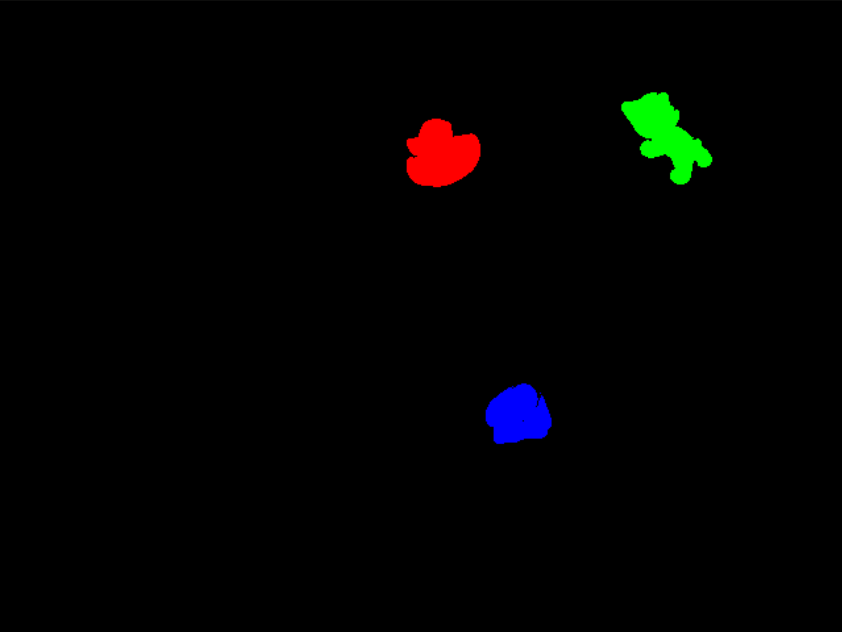
\includegraphics[height=3.5cm]{1_uncertain_seg}}
  \subcaptionbox{模型对齐\label{fig:uncertain_coordinate}}{%  
    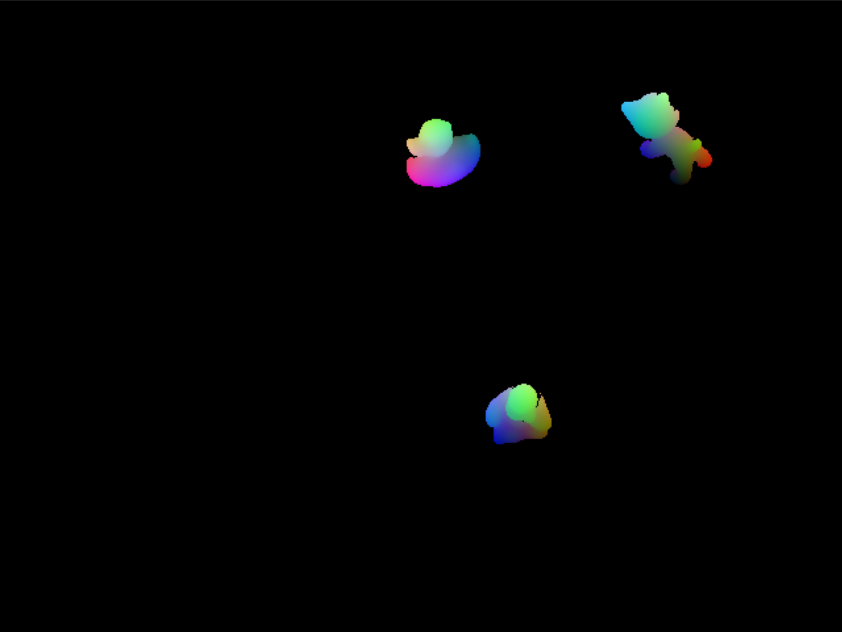
\includegraphics[height=3.5cm]{1_uncertain_coordinate}\hspace{0.15em}
    }%\vskip0.3cm
  \subcaptionbox{姿态估计\label{fig:uncertain_pos}}{%    
    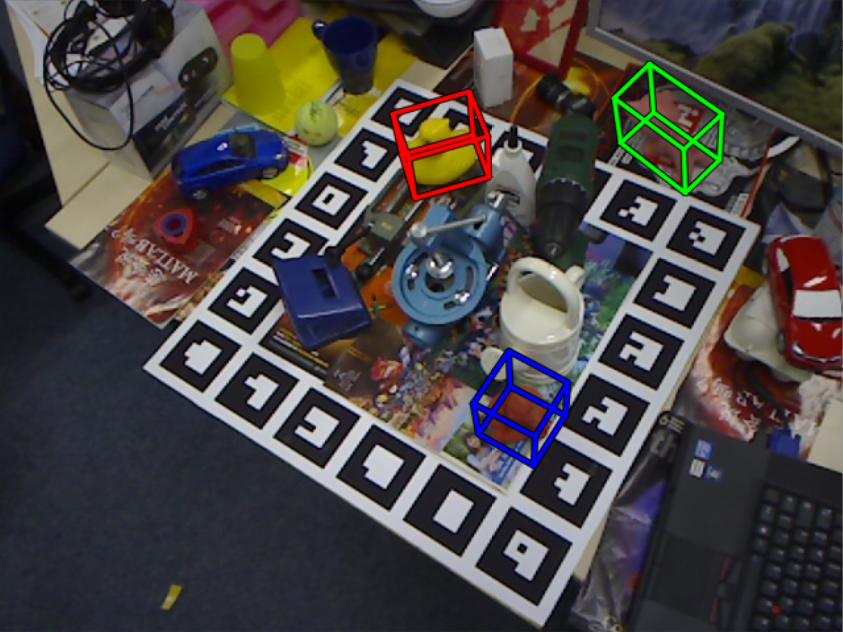
\includegraphics[height=3.5cm]{1_uncertain_pose}}
  \caption{随机森林姿态估计算法}
  \label{fig:uncertain_pose_estimation}
\end{figure}


\subsection{目标物体位置姿态追踪研究现状}
\label{sec:tracking_status}
基于特征点的目标位姿追踪系统已具备足够的准确性以及鲁棒性,该类方法受益于特征点提取匹配算法的发展而取得了不错的效果\cite{VacchettiStableRealtime3d2004}。如图~\ref{fig:feature_match}~所示,通过与事先输入的图片
进行特征点匹配以计算当前帧图片中目标物体的位姿,在一定场合中效果良好。
但该类算法对目标物体位姿追踪的精度受特征点匹配的准确性影响较大,因此易受背景复杂度、相机内参、光照变化等影响,
在复杂场景中位姿判定失败率高。为求结果稳定精确,需匹配大量特征点并进行联合优化,计算速度减慢但准确度提升,使用部分特征点匹配的方法在存在遮挡的情况下也能取得了不错的效果\cite{ParkMultiple3dObject2008}。


\begin{figure}[t]
  \centering
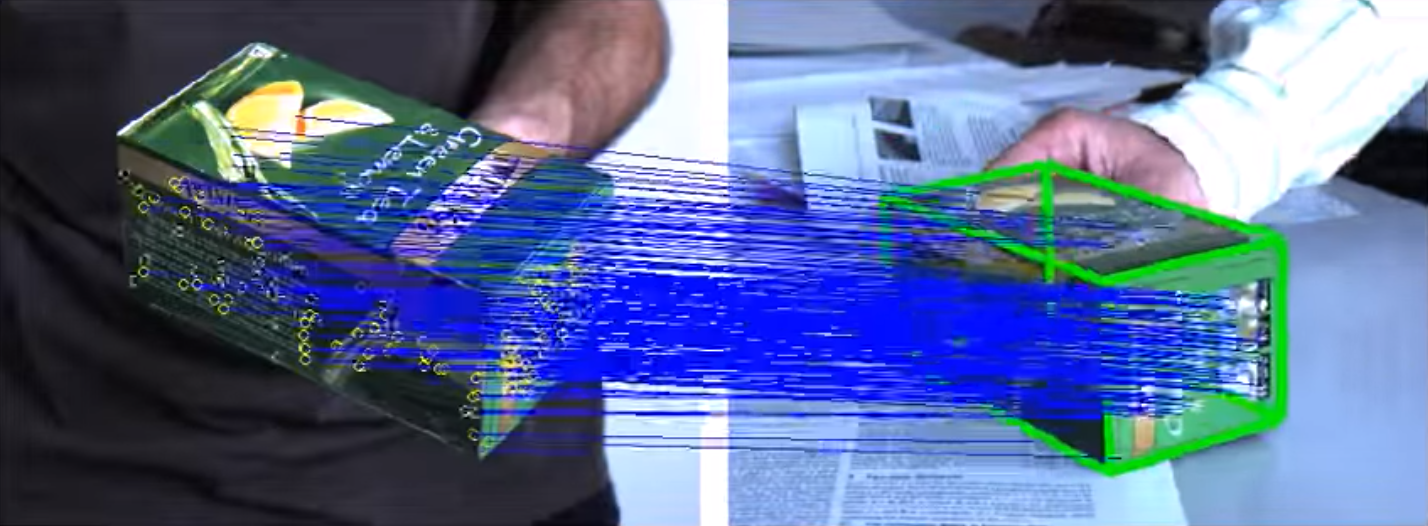
\includegraphics[height=5cm]{1_feature_match}
  \caption{特征点匹配追踪算法}
  \label{fig:feature_match}
\end{figure}


但对于表面纹理贫乏、无法提取特征点的目标对象或场景,上述方法将不再适用。
针对贫纹理对象发展出一类基于物体边缘或轮廓的匹配方法。最早的边缘匹配位姿追踪算法 RAPID\cite{HarrisRAPIDaVideoRate1990}于1990年就被提出,该方法通过将 3D 模型的边缘点映射到 2D 图像并将模型轮廓点与图像中的边缘点对齐,以追踪目标物体的位姿。随后出现很多改进算法,Eric Marchand~等人\cite{Marchand2D3DModelbased2001,ComportRealtimeTrackerMarkerless2003}使用卷积核函数提取
模型轮廓方向信息,通过方向信息匹配图像边缘与模型轮廓实现姿态追踪和定位;Harald Wuest~等人\cite{WuestAdaptiveLineTracking2005}于 2005 年使用多边缘假设方法,通过匹配多组图像边缘寻优的方法,提高追踪的精度,但算法计算耗时较长。
基于 3D-2D 的匹配关系,将物体轮廓进行旋转平移以求与图像边缘配准,最后计算模型的旋转矩阵与平移向量以实现目标物体的位姿追踪的方法
能够在环境简单、物体轮廓明显、无遮挡的场景中取得不错的效果,但该类算法仍是基于离散点的匹配,无法从轮廓整体进行寻优,因此在配准过程中容易陷入局部极小值,在出现较大追踪误差后无法还原,导致追踪失败。山东大学计算机科学与技术学院秦学英教授
于 2015 年开始研究全局优化的方法寻找物体轮廓与图像边缘的最优配准关系,提高了配准的精确度与鲁棒性,并且使用前后景分割的方法加快了轮廓线的提取过程,算法提升效果显著\cite{WangGlobalOptimalSearching2015,ChenHunHeXianShiZhongDeXuShiRongHeYuRenJiZhiNengJiaoRong2016,WangPoseOptimizationEdge2017}。

\section{主要研究内容和技术路线}
\label{sec:problem}
目标物体位置姿态追踪系统在贫纹理对象的应用中仍存在很多待解决的问题,如:
\begin{enumerate}[{(}1{)}]
\item 针对贫纹理对象的位姿真值数据库尚不完善,对物体位姿的测量误差较大,缺少必要的数据用于算法的学习和测试;
\item 基于物体边缘轮廓的检测与姿态估计算法精度较低、复杂度较高,需要进一步提高算法的实时性与准确性;
\item 现有算法对于背景复杂、存在遮挡等情况下的追踪效果欠佳,对环境边缘噪声的干扰缺乏鲁棒性。
\end{enumerate}

本文将针对现有目标物体位置姿态数据库中存在的问题,利用计算机图形学(Computer Graphics,简称CG)方法建立对应物体的位姿真值数据库,提供一套基于 CG 渲染技术的多背景、多场合目标物体移动
与姿态变换真值数据库,并对位姿真值与场景图片进行匹配验证,构造位姿数据库用于后续检测与追踪方法的学习与测试;
针对贫纹理物体的检测问题,本文使用学习算法检测并估计图像中目标物体的位姿,依靠 CG 渲染数据库进行该类算法的学习与评价,提高检测的准确度与
姿态估计的精度,并研究加快算法运行速度的途径与方法;
针对贫纹理物体姿态追踪问题,本文将使用基于轮廓对齐的方法,结合匹配寻优算法解算物体位姿,并设计追踪评价函数,依据评价函数改变追踪策略,改善追踪系统性能。
所研究系统将达到如下指标:
\begin{enumerate}[(1)] 
  \item 系统能够检测并追踪目标物体相对于相机的平移向量,向量方向误差小于~2$^\circ$,位置距离误差小于位置真值的~5\%。
  \item 系统能够检测并追踪目标物体相对于相机的姿态,各轴角度误差小于~2$^\circ$。
  \item 提供一套由 CG 渲染技术自动生成目标物体位姿真值数据库的技术,并为各模块提供相应数据集以及测试真值。
  \end{enumerate}

结合研究内容,完成目标物体位姿检测与追踪系统的理论研究、系统实现以及测试实验与分析,技术路线如图 \ref{fig:tech_path} 所示。总结研究问题,依据技术路线的规划,本文的章节安排如下所示:

第 1 章:查阅国内外“贫纹理物体检测”、“姿态估计”以及“位姿追踪”等相关领域研究文献及技术资料,对基于模型的边缘追踪方法、物体姿态解算算法的发展过程和研究现状作了详细调研和综述,
为相关研究工作的开展提供必要性依据,并在明确研究对象的基础上,提炼存在的科学问题,确定研究方法、目标和技术路线。

第 2 章:研究基于模型的贫纹理物体位姿追踪算法,构造模型与场景图像匹配的目标函数,深究目标函数的优化方法,通过寻优方法得到模型与场景边缘图像的最优匹配,以解算物体相对于
相机坐标系的旋转矩阵以及平移向量。讨论物体追踪中出现的遮挡问题,研究利用调整模型匹配点优化权重的方法以解决该问题,提高系统的稳定性以及鲁棒性。

第 3 章:使用追踪算法获取真实场景中的目标物体位置以及姿态,构建检测数据库以及平移向量数据库,以备后续对机器学习算法中的模型进行训练。
研究使用~3D~渲染引擎生成位姿真值数据库的方法,用以代替传统的数据采集方式,利用三维建模软件搭建实验场景,构建不同角度、背景、物体大小的目标位姿真值数据库,
用以对追踪算法进行精度测试。

第 4 章:研究基于机器学习方法的贫纹理物体检测方法,并通过检测结果以及图像信息估计目标位姿,实现自动初始化系统,为追踪算法提供位姿初值。
还将讨论初始化系统以及追踪系统的整合问题,研究两种算法的切换逻辑,实现系统对目标丢失后重新初始化,加强追踪的鲁棒性。

第 5 章:分别对本文所提的初始化系统与位姿追踪系统进行测试。其中初始化系统将使用分模块的测试方法,对初始化的各流程进行单独测试,以分析初始化各流程的精度以及误差,讨论误差产生的原因以及提高方法;
对追踪系统的测试将分为实物场景测试、真实数据库测试以及遮挡测试,分别测试追踪算法的背景鲁棒性、精度以及抗干扰能力。

第 6 章:总结本文的研究工作,指出初始化系统与位姿追踪系统研究工作中存在的不足和改进空间,并为后续研究提出若干研究方向。

\begin{figure}[!p]
  \centering
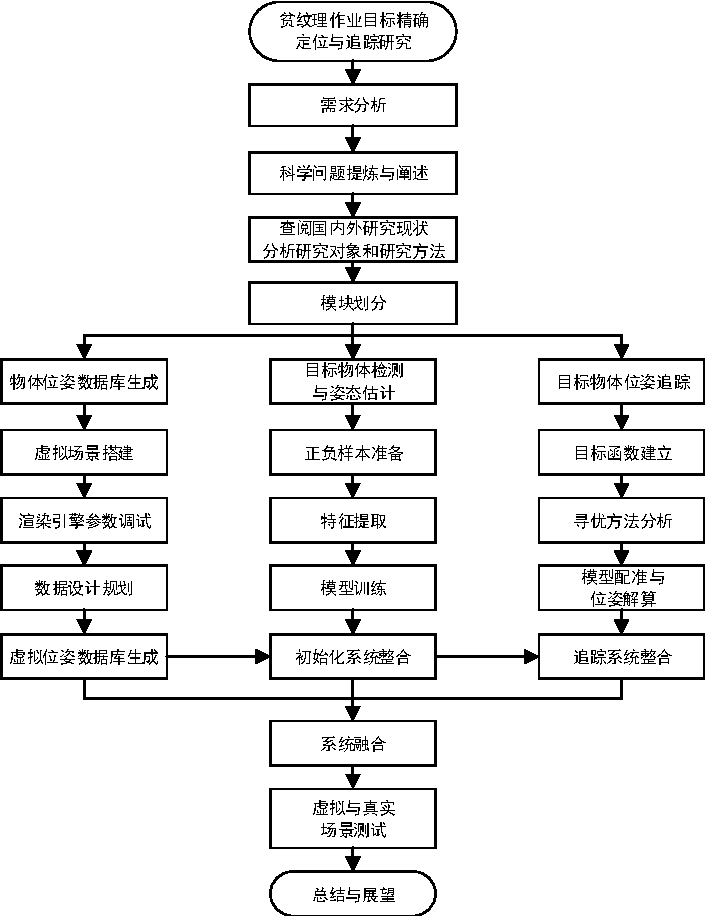
\includegraphics[width=16cm]{1_tech_path_mine}
  \caption{技术路线图}
  \label{fig:tech_path}
\end{figure}

